\documentclass{beamer}
\usetheme{Madrid}
\usepackage[utf8]{inputenc}
\usepackage{graphicx}
\title{Roots of Niels Bohr’s Thought}
\author{Hans Halvorson}
\date{}
\begin{document}
\frame{\titlepage}
\begin{frame}{Roots of Niels Bohr’s Thought}
\begin{itemize}
  \item Hans Halvorson
\end{itemize}
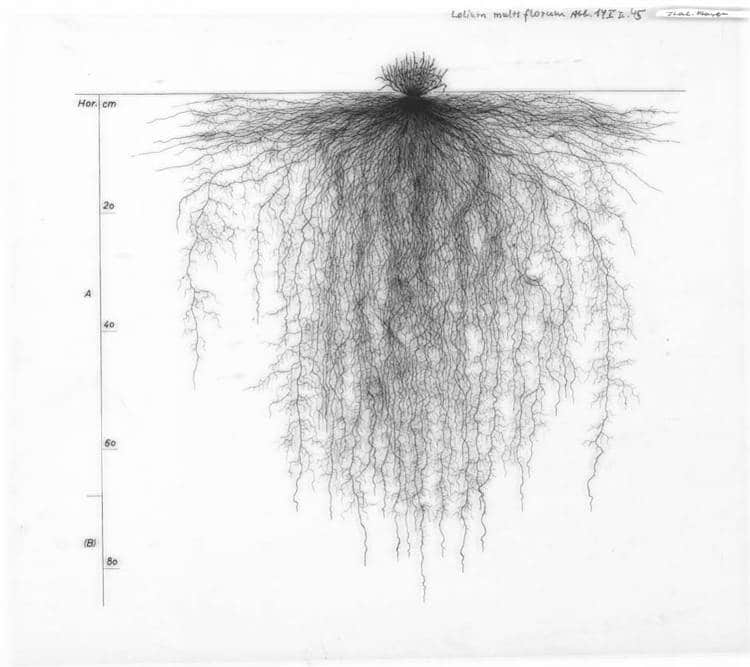
\includegraphics[width=0.9\linewidth]{slide1_img1.jpg}
\end{frame}
\begin{frame}{Not so secret: Trouble with physics}
\begin{itemize}
  \item 2
\end{itemize}
% \includegraphics[width=0.9\linewidth]{slide2_img2.wmf}
\end{frame}
\begin{frame}{Pointing the finger: Bohr was a positivist}
\begin{itemize}
  \item “Without doubt, Bohr’s philosophical views have shaped the way generations of physicists think about quantum mechanics, but they have also, in the eyes of an increasing number, discouraged and stifled progress.” (Jim Al-Khalili, 2020, p 122)
  \item 3
\end{itemize}
\end{frame}
\begin{frame}{Pointing the finger: Bohr was unclear}
\begin{itemize}
  \item “While imagining that I understand the position of Einstein, … I have very little understanding of the position of his principal opponent, Bohr.
… Indeed, I have very little idea what this means. I do not understand in what sense the word ‘mechanical’ is used …. I do not know what the italicized passage means.” (John Bell, Bertlmann’s Socks)
  \item 4
\end{itemize}
\end{frame}
\begin{frame}{Pointing the finger: Science has forgotten its humanist roots}
\begin{itemize}
  \item 5
\end{itemize}
\end{frame}
\begin{frame}{Catherine Chevalley}
\begin{itemize}
  \item “Bohr’s ideas were not located in their proper background, either scientific or philosophical, until quite recently.”
  \item 6
\end{itemize}
\end{frame}
\begin{frame}{Filosofisk smagsprøve}
\begin{itemize}
  \item “Every unambiguous communication about the state and activity of our mind implies of course a separation between the content of our consciousness and the background loosely referred to as ‘ourselves’ but any attempt at exhaustive description of the richness of conscious life demands in various situations a different placing of the section between subject and object.”
  \item 7
\end{itemize}
\end{frame}
\begin{frame}{“In order to illustrate this important point, I shall quote a Danish poet and philosopher, Poul Martin Møller, who lived about a hundred years ago and left behind an unfinished novel called “The Adventures of a Danish Student”, in which the author gives a remarkably vivid and suggestive account of the interplay between the various aspects of our position . . .” (Bohr 1960, p 65)}
\begin{itemize}
  \item 8
\end{itemize}
\end{frame}
\begin{frame}{Bell, Al Khalili, and their ilk are hamstrung. They cannot see the root system.}
\begin{itemize}
  \item 9
\end{itemize}
\end{frame}
\begin{frame}{Bohr as Kantian?}
\begin{itemize}
  \item 10
  \item “Bohr’s interpretation was rooted into every detail of the long genesis of atomic physics, and it was formulated within the philosophical language that developed in the German culture starting with Kant.” (Catherine Chevalley)
\end{itemize}
\end{frame}
\begin{frame}{Bohr as Kierkegaardian?}
\begin{itemize}
  \item “There can be no doubt that the Danish precursor of modern existentialism and neo-orthodox theology, Søren Kierkegaard, through his influence on Bohr, affected also the course of modern physics to some extent.” 
(Jammer 1966, p 173)
  \item 11
\end{itemize}
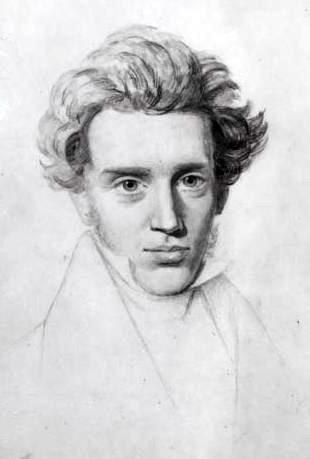
\includegraphics[width=0.9\linewidth]{slide11_img3.jpg}
\end{frame}
\begin{frame}{Bohr’s Defender}
\begin{itemize}
  \item 12
\end{itemize}
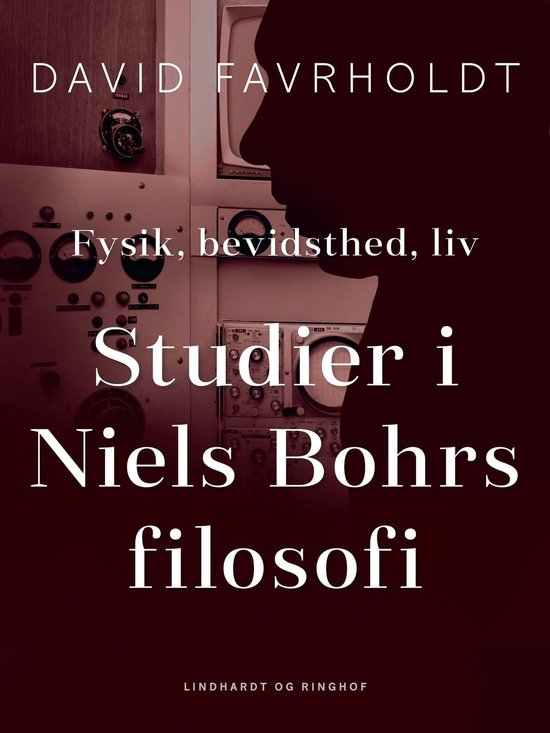
\includegraphics[width=0.9\linewidth]{slide12_img4.jpg}
% \includegraphics[width=0.9\linewidth]{slide12_img5.wmf}
\end{frame}
\begin{frame}{Bohr as great philosopher}
\begin{itemize}
  \item “Of course, a lot has already been written about Bohr's philosophy, but unfortunately not many people have been able to see the depth of it and its new vision when it comes to traditional philosophical issues.” (Favrholdt, FNB)

“I consider Niels Bohr to be one of the greatest thinkers in human history.”(Favrholdt, FNB)
  \item 13
\end{itemize}
\end{frame}
\begin{frame}{Ideas ex Nihilo}
\begin{itemize}
  \item “Do we have any reason at all to believe that Bohr was influenced by Kierkegaard’s philosophy? The answer is in the negative.” (NBFB, p 62)

“If we wish to speak of an influence in this case, the influence is actually an antithetical one. And if in his first reading of Kierkegaard Bohr reacted against his ideas, then the roots of his own view must be sought elsewhere.” (NBFB, p 54)
  \item 14
\end{itemize}
\end{frame}
\begin{frame}{Ideas ex Nihilo}
\begin{itemize}
  \item “Neither Kierkegaard nor Høffding mentions an arbitrary dividing line between subject and object. Only in Poul Martin Møller’s writings do we find this idea.” (NBPB, p 57)

“It seems that [Harald] Høffding played little or no part as regards the formulation of Bohr's specific contribution to philosophy.”
  \item 15
\end{itemize}
\end{frame}
\begin{frame}{Contra Favrholdt, the proper way to understand “influence” on Niels Bohr’s thought is via transformation.
Not direct transmission from texts, but more like absorption from the cultural soil.
Kierkegaard’s ideas are in the mix – as are the ideas of many other 18th and 19th century thinkers.}
\begin{itemize}
  \item 16
\end{itemize}
\end{frame}
\begin{frame}{Working Backwards}
\begin{itemize}
  \item Bohr
The moveable line between subject and object 
“Unambiguous”
Complementarity is an objective description
Classical concepts 
Analysis and synthesis
Mechanism versus vitalism
Free will 
No “God’s eye view”
  \item 17
\end{itemize}
\end{frame}
\begin{frame}{Bohr’s proximal philosophical influences}
\begin{itemize}
  \item Bohr read Stadier paa Livets Vei
Bohr’s father was friends with Harald Høffding
Bohr took a year of Filosofikum (teacher was Høffding)
Bohr’s father took a year of Filosofikum (teacher Rasmus Nielsen’s)
  \item 18
\end{itemize}
\end{frame}
\begin{frame}{Harald Høffding (1843-1931)}
\begin{itemize}
  \item 19
\end{itemize}
% \includegraphics[width=0.9\linewidth]{slide19_img6.wmf}
\end{frame}
\begin{frame}{Rasmus Nielsen (1809-1884)}
\begin{itemize}
  \item 20
\end{itemize}
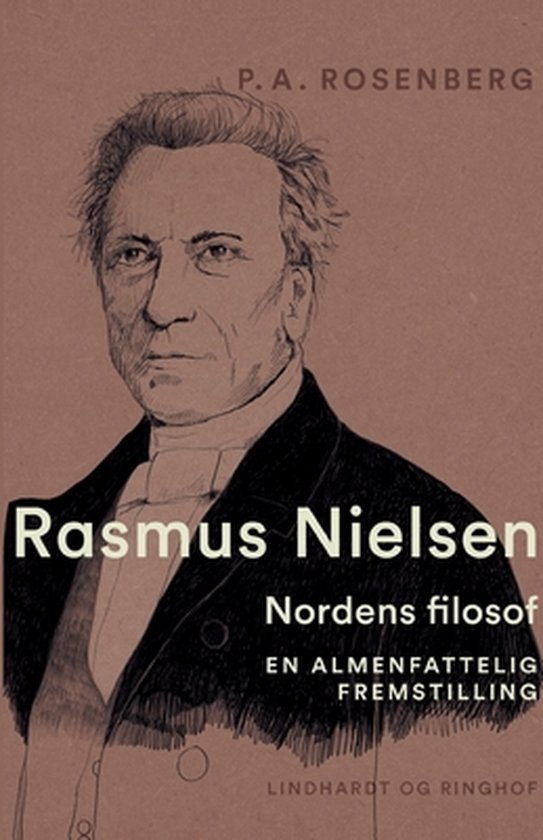
\includegraphics[width=0.9\linewidth]{slide20_img7.jpg}
\end{frame}
\begin{frame}{A single data point in English}
\begin{itemize}
  \item SK and RN were contemporaries and friends for a couple of years. Then SK accused RN of stealing his ideas.


			See Jon Stewart, “Rasmus Nielsen: From the Object of ‘Prodigious Concern’ to a ‘Windbag’.”
  \item 21
\end{itemize}
\end{frame}
\begin{frame}{The once-famous Rasmus Nielsen}
\begin{itemize}
  \item “No one who studies the life of the mind in nineteenth-century Denmark, will be able to skip over [Nielsen’s] great philosophical writings, and everyone who got to hear his lectures at the university will remember him as a great awakener and a rare personality.” (Brandes 1899)
  \item 22
\end{itemize}
\end{frame}
\begin{frame}{The once-famous Rasmus Nielsen}
\begin{itemize}
  \item Nielsen taught several generations of the most distinguished scientists, philosophers, and humanists in Denmark
Taught Filosofikum from 1841 to 1882
Published thousands of pages of philosophy
Nothing of Nielsen’s has been translated into a “world language”
  \item 23
\end{itemize}
\end{frame}
\begin{frame}{Nielsen’s students}
\begin{itemize}
  \item 24
  \item J. Lange 1859
  \item G. Brandes 1859
  \item H. Høffding 1861
\end{itemize}
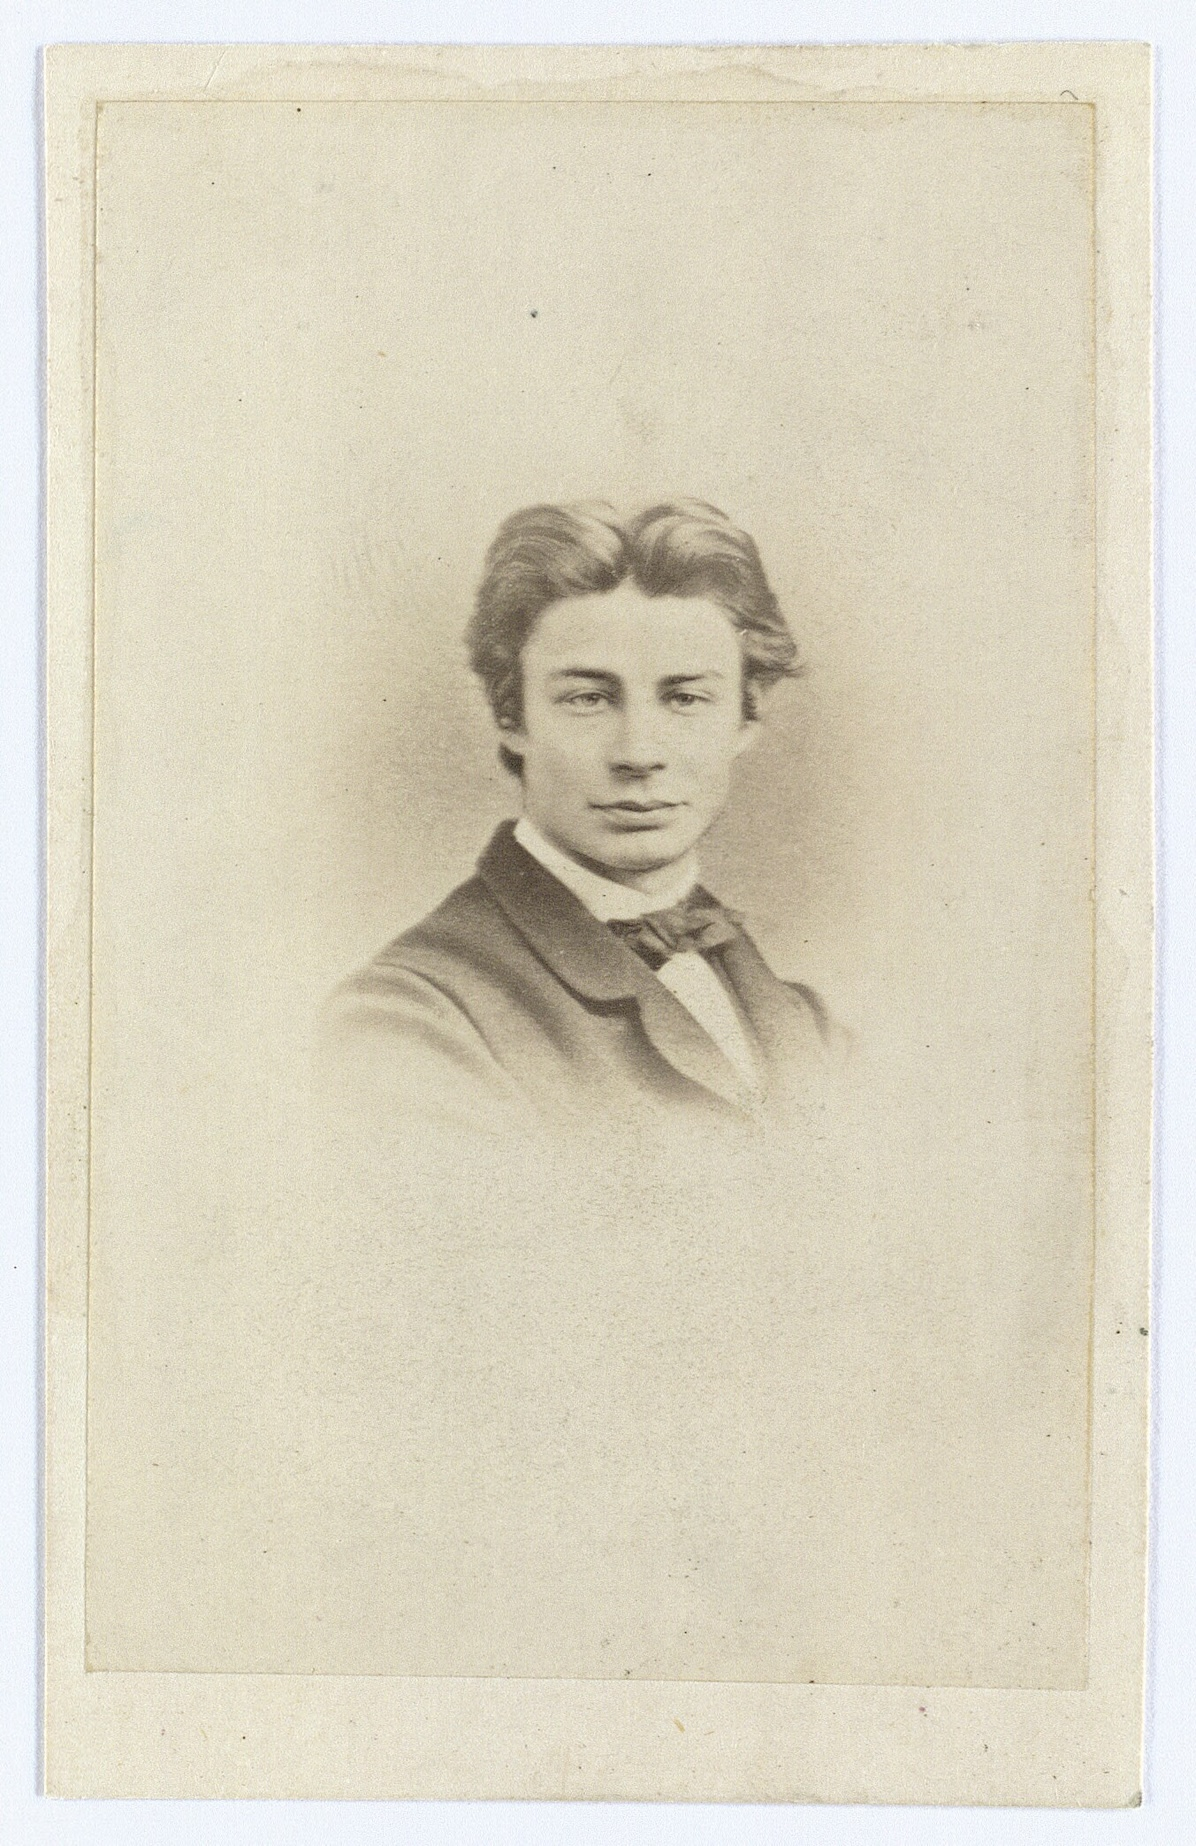
\includegraphics[width=0.9\linewidth]{slide24_img8.jpg}
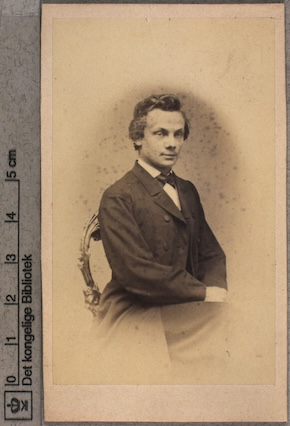
\includegraphics[width=0.9\linewidth]{slide24_img9.jpg}
\end{frame}
\begin{frame}{“At first it was Rasmus Nielsen, whose enthusiastic references to Kierkegaard and whose rousing eloquence had the greatest influence on me.” (Høffding 1909)}
\begin{itemize}
  \item 25
\end{itemize}
\end{frame}
\begin{frame}{Høffding, Danske Filosoffer}
\begin{itemize}
  \item 26
\end{itemize}
\end{frame}
\begin{frame}{“You were originally a disciple of Rasmus Nielsen. Like others, you were subject to the attraction of this deft, sparkling virtuoso of intellectual skill, this Ole Bull of philosophy with his spark of life, against whom posterity is so cold because he was far too prevalent in his time.” 
(G. Brandes, Tale for H. Høffding, 1903)}
\begin{itemize}
  \item 27
\end{itemize}
\end{frame}
\begin{frame}{28}
\begin{itemize}
  \item C. Bohr 1874
  \item K. Kroman 1868
\end{itemize}
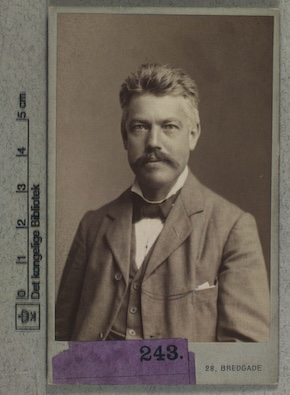
\includegraphics[width=0.9\linewidth]{slide28_img10.jpg}
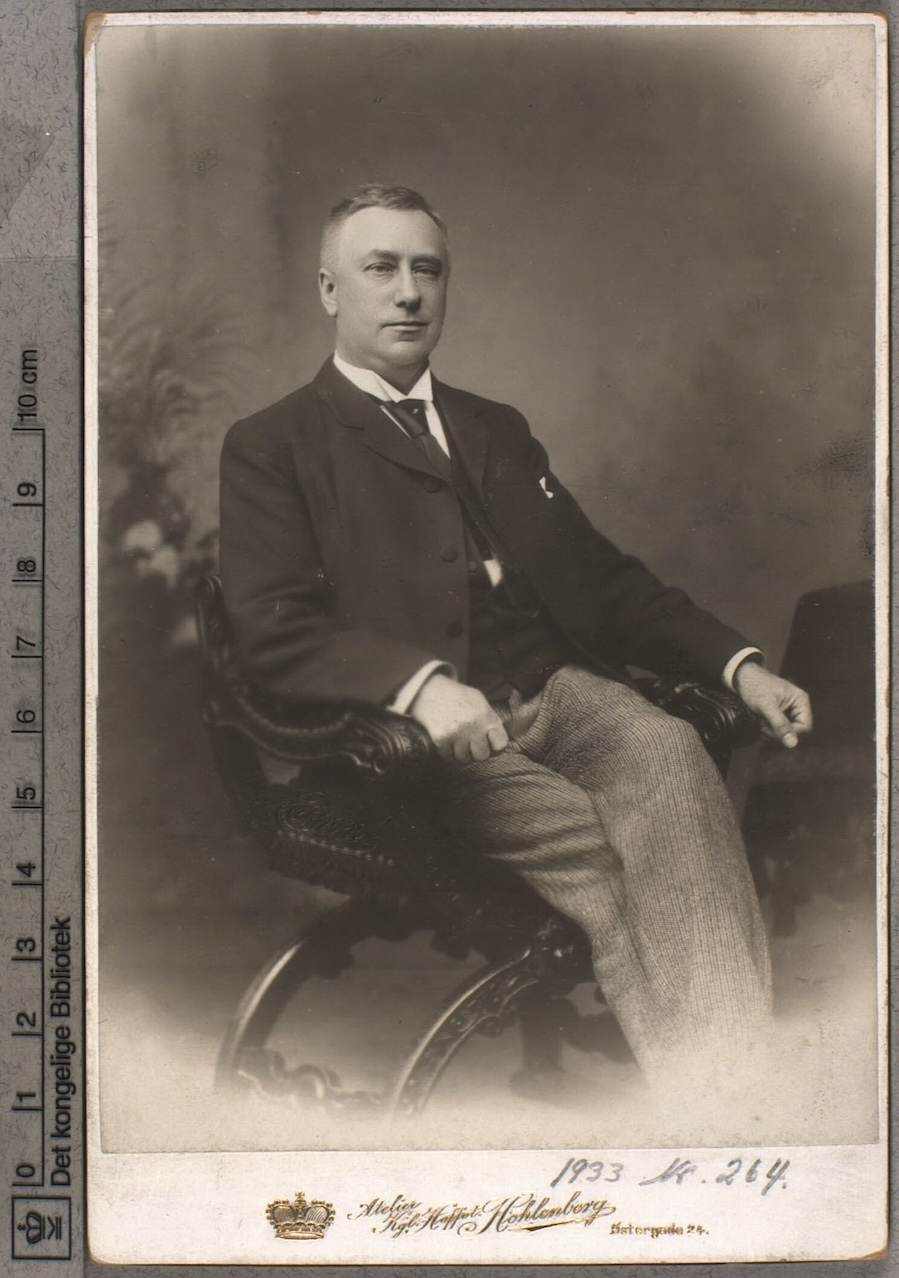
\includegraphics[width=0.9\linewidth]{slide28_img11.jpg}
\end{frame}
\begin{frame}{Who was Rasmus Nielsen?}
\begin{itemize}
  \item 1809 bondefødt in Rorslev, Middelfart
1820 intellectual talents recognized by local priest 

1829 begins studies at Viborg katedralskole 

	1830 SK matriculates at KU
  \item 29
\end{itemize}
\end{frame}
\begin{frame}{Who was Rasmus Nielsen?}
\begin{itemize}
  \item 1832 graduated Viborg katedralskole 

1837 teologisk embedseksamen
	1839 SK’s journal: satirical remarks about RN
  \item 30
\end{itemize}
\end{frame}
\begin{frame}{Nielsen’s Hegelian Period}
\begin{itemize}
  \item 1840 PhD: De speculativa historiæ sacræ tractandæ method

	1841 SK PhD: Begrebet Ironi

1841 RN appointed chair of moral philosophy (Poul Møller’s chair)

	1842 SK remarks satirically about RN’s unfinished system in 		            Fædrelandet

1845 Den Logiske Propædeutik
  \item 31
\end{itemize}
\end{frame}
\begin{frame}{Relationship with Kierkegaard}
\begin{itemize}
  \item 1846 SK. Afsluttende Uvidenskabelig Efterskrift

1848 SK and RN begin taking regular walks together. SK: RN is the only one of the younger thinkers in Denmark who “may amount to something”.

1849 RN. Evangelietroen og den moderne Bevidsthed 

	SK: “The writings are plundered in many ways . . . And then 	my conversations!”
  \item 32
\end{itemize}
\end{frame}
\begin{frame}{Relationship with Kierkegaard}
\begin{itemize}
  \item 1849 Martensen. Den Christelige Dogmatik

1849 RN. Mag. S. Kierkegaards “Johannes Climacus” og Dr. H. Martensens “Christelige Dogmatik.” En undersøgende Anmeldelse.

1850 RN. Evangelietroen og Theologien
  \item 33
\end{itemize}
\end{frame}
\begin{frame}{Nielsen’s Scientific Turn}
\begin{itemize}
  \item 1855 Om Theologiens Naturbegreb med særligt Hensyn til  	Malebranche: De la recherche de la verité

1857 Philosophisk Propædeutik i Grundtræk

1857 Philosophie og Mathematik. En propædeutisk Afhandling

1859 Mathematik og Dialektik
  \item 34
\end{itemize}
\end{frame}
\begin{frame}{“As my recent writings show, it has been my goal, for several years, to clarify and demonstrate the relationship between philosophy and the separate sciences as comprehensively as possible. The future of philosophy depends in an essential way on a thorough understanding and accurate determination of this relationship.” (1864, p 18)}
\begin{itemize}
  \item 35
\end{itemize}
\end{frame}
\begin{frame}{The second battle about faith and reason}
\begin{itemize}
  \item 1864  Nielsen. Grundideernes Logik.
	“Tro og Viden er uensartede Principper”.

1866  Brandes. Dualismen i vor  nyeste Philosophie

1866  Høffding. Philosophie og  Theologie

1867  Nielsen. Om ‘Den Gode Villie’ som Magt i Videnskaben
  \item 36
\end{itemize}
\end{frame}
\begin{frame}{The so-called Heisenberg cut}
\begin{itemize}
  \item Bohr talked about a moveable boundary (skillelinien) between subject and object
Contemporary physicists are confused
John Bell: “The shifty split”
“The first charge against 'measurement', in the fundamental axioms of quantum mechanics, is that it anchors there the shifty split of the world into ‘system’ and ‘apparatus’.” (Against Measurement)
  \item 37
\end{itemize}
\end{frame}
\begin{frame}{38}
\end{frame}
\begin{frame}{39}
\begin{quote}
“Ordinary language, by its use of such words as thoughts and sentiments, admits typical complementary relation between conscious experiences implying a different placing of the section line between the observing subject and the object on which attention is focused.”
\end{quote}
\end{frame}
\begin{frame}{“In fact, the varying separation line between subject and object, characteristic of different conscious experiences, is the clue to the consistent logical use of such contrasting notions as will, conscience and aspirations, each referring to equally important aspects of the human personality.” (Bohr 1953, pp 389-390)}
\begin{itemize}
  \item 40
\end{itemize}
\end{frame}
\begin{frame}{“In emphasizing the necessity of paying proper attention to the placing of the object-subject separation in unambiguous communication, the modern development of science has created a new basis for the use of such words as knowledge and belief.” (Bohr 1955, p 61)}
\begin{itemize}
  \item 41
\end{itemize}
\end{frame}
\begin{frame}{42}
\end{frame}
\begin{frame}{Høffding, Erkendelsesteori}
\begin{itemize}
  \item 43
\end{itemize}
\end{frame}
\begin{frame}{Høffding, Erkendelsesteori}
\begin{itemize}
  \item 44
\end{itemize}
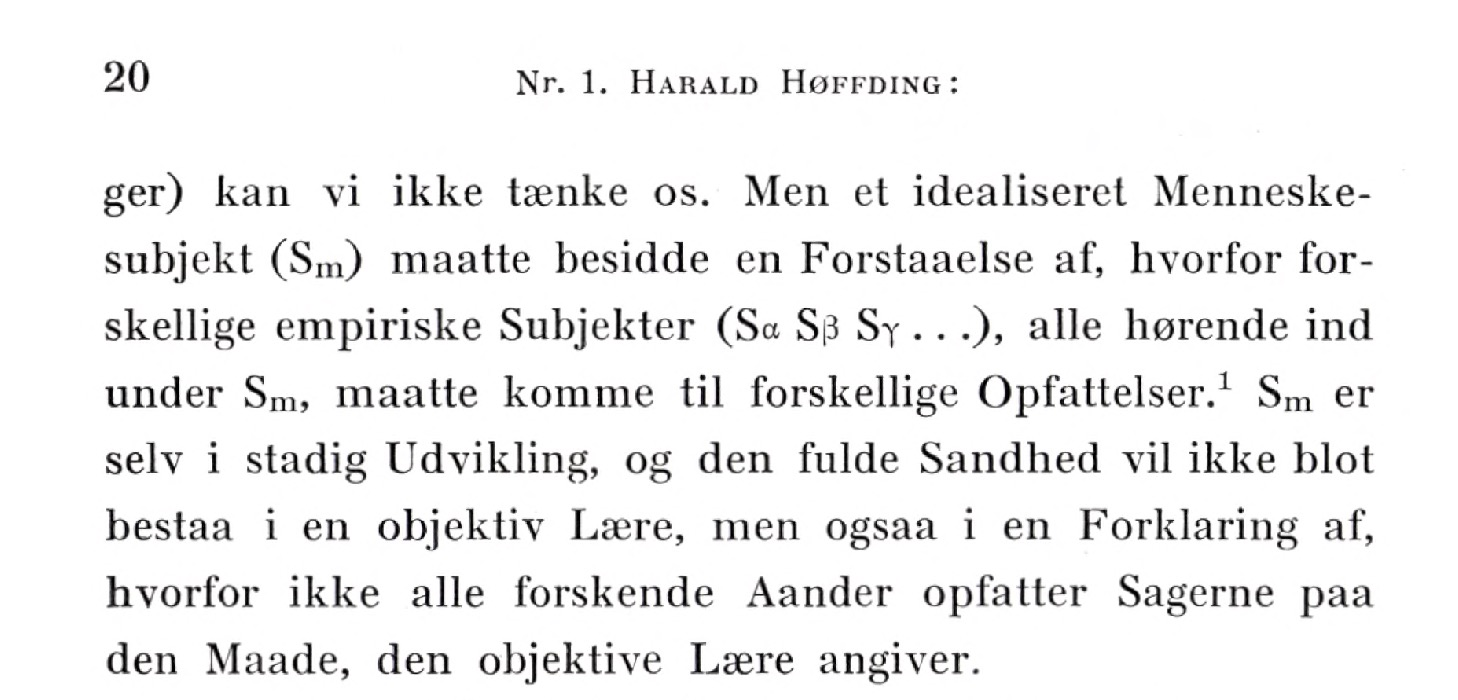
\includegraphics[width=0.9\linewidth]{slide44_img12.jpg}
\end{frame}
\begin{frame}{Høffding, Den Menneskelige Tanke (1910)}
\begin{itemize}
  \item 45
\end{itemize}
\end{frame}
\begin{frame}{Why has Nielsen been neglected}
\begin{itemize}
  \item Abstract and heavy writing style
Challenged scientists’ authority
On the wrong side of Det Moderne Gennembrud
  \item 46
\end{itemize}
\end{frame}
\begin{frame}{”Komplementaritetsfilosofien, som er Bohrs højst personlige og meget københavnske sammenfatning af kvantemekanikkens erkendelsesteori, stort set ikke er blevet forstået af det internationale fysikersamfund.”
 Peder Voetmann Christensen, Springet fra København, Information,  7. okt 1985}
\begin{itemize}
  \item 47
\end{itemize}
\end{frame}
\begin{frame}{”Men hvorfor prøver man så ikke at forstå den filosofi, som førte til Bohrs sikre forudsigelser? Det var jo ikke en krystalkugle, men logisk tænkning, som lå bag.
Jeg tror, at svaret skal søges i, at Bohrs filosofi netop er meget københavnsk. Den bygger på nogle forudsætninger, en særlig begrebslogik, som er udviklet i 1800-tallets København, men som ikke specielt har noget med fysik at gøre.”}
\begin{itemize}
  \item 48
\end{itemize}
\end{frame}
\begin{frame}{49}
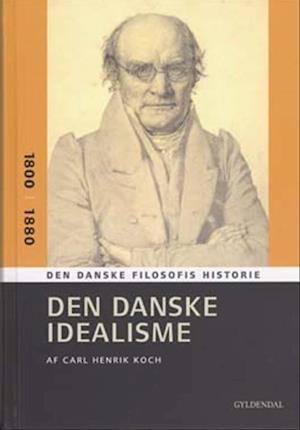
\includegraphics[width=0.9\linewidth]{slide49_img13.jpg}
\end{frame}
\begin{frame}{50}
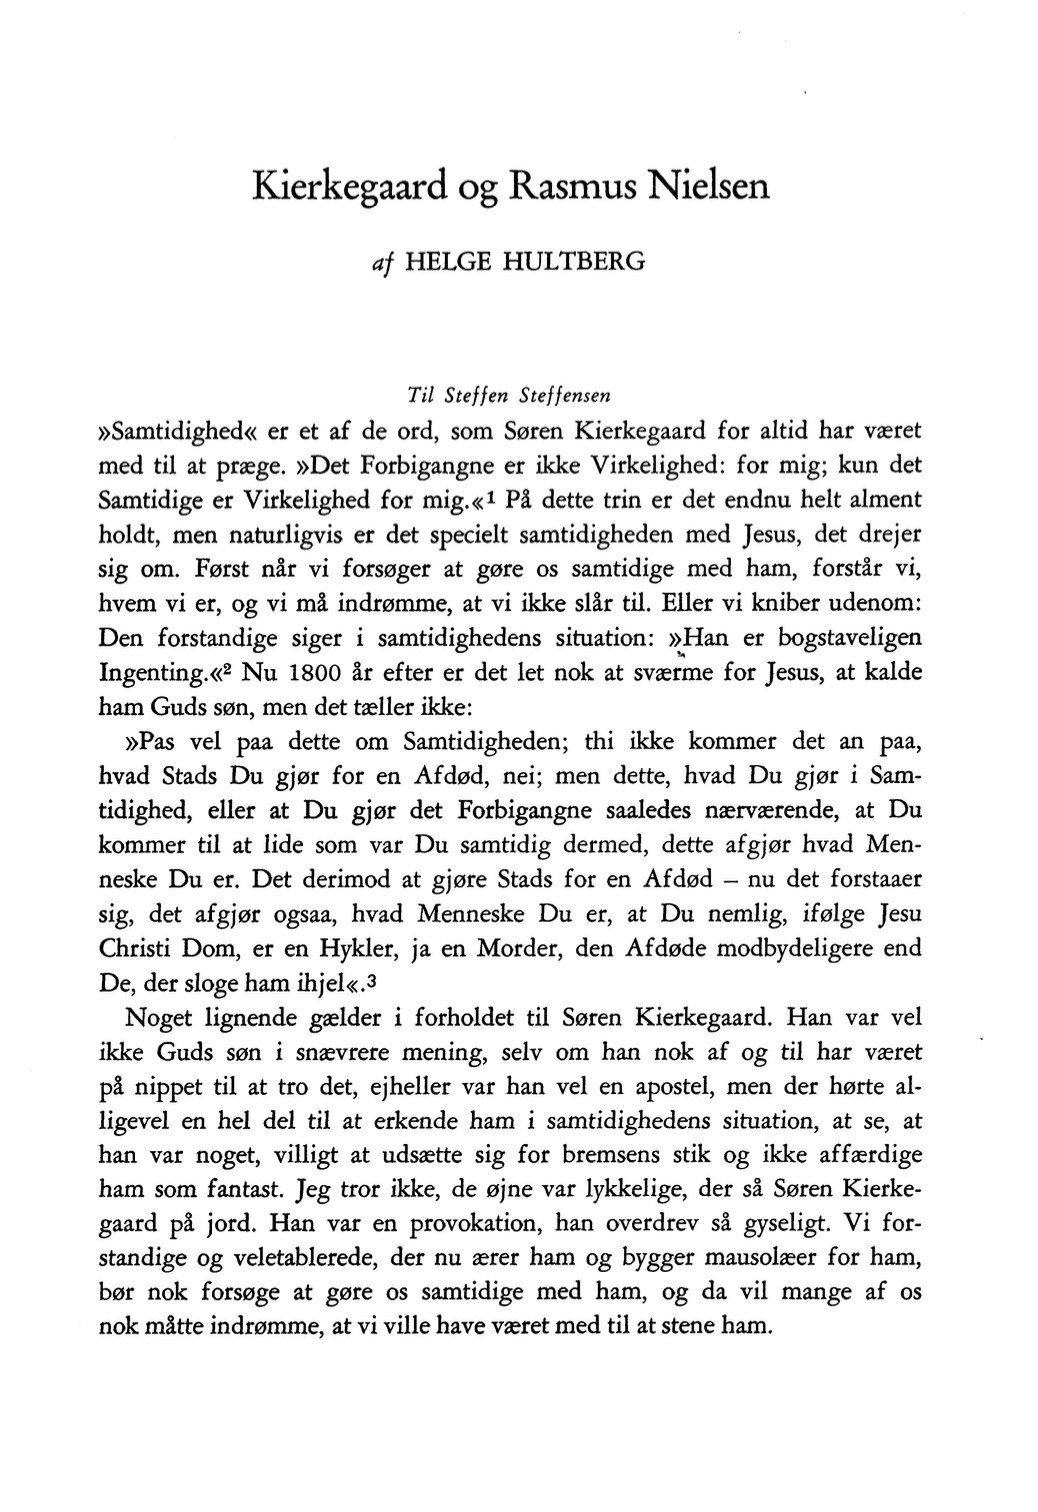
\includegraphics[width=0.9\linewidth]{slide50_img14.jpg}
\end{frame}
\begin{frame}{51}
\end{frame}
\end{document}
%%% Local Variables:
%%% mode: latex
%%% TeX-master: t
%%% End:
